%!TEX root = ../template.tex
%%%%%%%%%%%%%%%%%%%%%%%%%%%%%%%%%%%%%%%%%%%%%%%%%%%%%%%%%%%%%%%%%%%%
%% chapter4.tex
%% NOVA thesis document file
%%
%% Chapter with lots of dummy text
%%%%%%%%%%%%%%%%%%%%%%%%%%%%%%%%%%%%%%%%%%%%%%%%%%%%%%%%%%%%%%%%%%%%

\typeout{NT FILE chapter4.tex}%

\chapter{RPC}
\label{cha:RPC}

\epigraph{
	"What we observe is not nature itself, but nature exposed to our method of questioning."
}{Werner Heisenberg}
\epigraph{
	"The scientist is not a person who gives the right answers, but one who asks the right questions — and builds the tools to answer them."
}{Claude Lévi-Strauss (paraphrased)}
\epigraph{
	"Precision is not just about measurement — it is about insight."
}




\section{History of RPCs/ Introduction}

\section{Properties}
      
\section{Build (components, electronics, gas mixture, DAQ, etc.)}

\gls{DAQ}

\subsection{RPC Build}

\begin{itemize}
	\item Active area of 1550x1250 mm$^2$ = 1.9 m$^2$.
	\item Two modules composed 6 gap RPC glass stacks.
	\item Gas mixture of C2H2F4 (98\%) and SF6 (2\%).
	\item Readout strips 3 cm width (placed in the middle of the two modules).
	\item Readout in both sides of the strips
\end{itemize}

\begin{figure}
	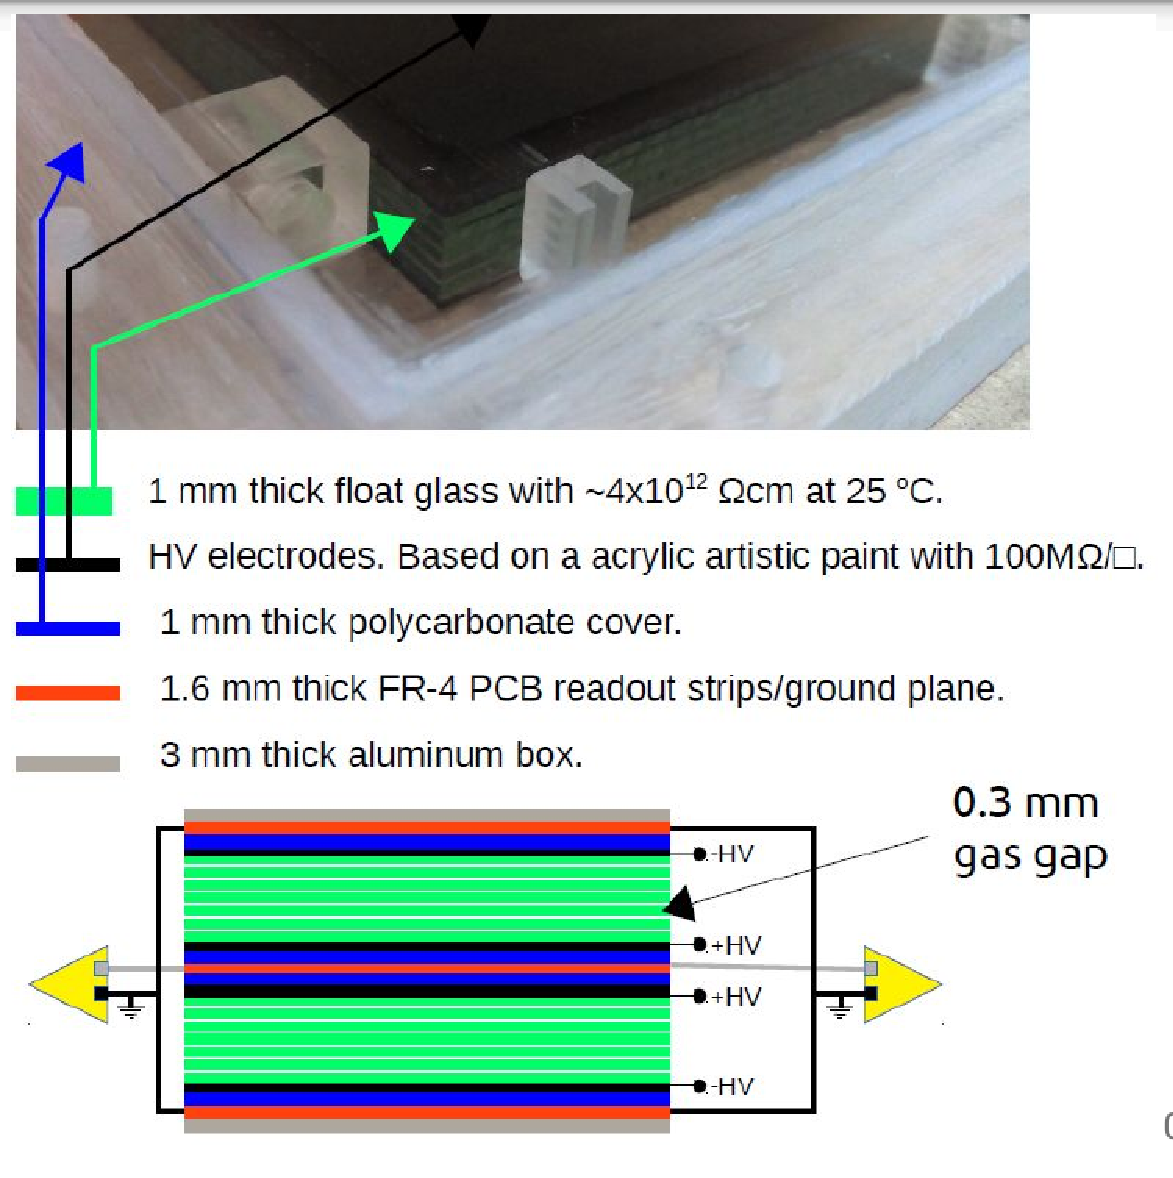
\includegraphics[width=\linewidth]{RPC Schematic}
	\caption{Schematic representation of the RPC.}
	\label{fig:RPCScheme}
\end{figure}

\subsection{RPC Electronics}

\subsection{RPC Gas Mixture}

\subsubsection{Pressure}

The working pressure inside the chamber is lower than atmospheric pressure. This ends up being helpful because the atmospheric pressure itself compresses the RPC and makes everything tidy, aligned and without gaps.


\subsubsection{Understanding the Role of the Gas Mixture in Resistive Plate Chambers (RPCs)}

The gas mixture used in the Resistive Plate Chamber (RPC) at R3B consists of:

\begin{itemize}
	\item 98\% C$_2$H$_2$F$_4$ (Tetrafluoroethane, also known as R-134a, or Freon).
	\item 2\% SF$_6$ (Sulfur Hexafluoride).
\end{itemize}


This specific gas combination plays a critical role in ionization, charge transport, avalanche formation, and quenching mechanisms inside the RPC. Below, the physics behind each component and their contributions to RPC performance are presented.


\subsubsection{Role of C$_2$H$_2$F$_4$ (Tetrafluoroethane - Freon)}

Primary Function: Ionization Medium and Avalanche Formation

C$_2$H$_2$F$_4$ is the main working gas, meaning that it provides the environment in which the ionization and charge multiplication take place.

Key Physics:

\begin{enumerate}
	
	\item Ionization by Charged Particles
	\begin{itemize}
		\item When a charged particle (e.g., a proton, electron, or ion) passes through the RPC, it ionizes the gas molecules, creating free electrons and positive ions.
		\item The number of ionization events depends on the stopping power (dE/dx) of the particle.
	\end{itemize}
	\item Electron Acceleration and Avalanche Formation
	\begin{itemize}
		\item The electric field inside the RPC accelerates the free electrons, leading to electron impact ionization.
		\item This results in an avalanche process, where an initial electron triggers a chain reaction of ionization events.
		\item C$_2$H$_2$F$_4$ has a moderate first ionization energy (~11.7 eV), making it an efficient medium for this multiplication process.
	\end{itemize}
	\item High Electron Attachment and Low Diffusivity
	\begin{itemize}
		\item Unlike noble gases (which have high electron mobility), C$_2$H$_2$F$_4$ has moderate electron attachment properties.
		\item This prevents excessive diffusion of electrons, leading to more localized avalanches.
		\item The electron mean free path is controlled to ensure controlled charge multiplication.
	\end{itemize}
	
\end{enumerate}


Why C$_2$H$_2$F$_4$ is Used Instead of Noble Gases?

\begin{itemize}
	\item Noble gases like argon have too high a mobility, leading to excessive charge spread and loss of spatial resolution.
	\item C$_2$H$_2$F$_4$ is a polyatomic gas, meaning that it has multiple molecular vibrational modes, which help in absorbing excess energy and controlling the growth of the avalanche.
\end{itemize}


\subsubsection{Role of SF$_6$ (Sulfur Hexafluoride)}
Primary Function: Quenching Agent and Sparking Suppression

Although only 2\% of the mixture, SF$_6$ is crucial for ensuring that the detector operates in a controlled avalanche mode rather than a full electrical breakdown (streamer mode).

Key Physics:

\begin{enumerate}
	\item Electron Capture and Avalanche Control
	\begin{itemize}
		\item SF$_6$ is a strong electronegative gas, meaning it has a very high affinity for capturing free electrons.
		\item This limits the size of the avalanche, preventing uncontrolled charge growth.
		\item By capturing electrons, SF$_6$ reduces the risk of streamer formation, which would cause sparking and damage the RPC.
	\end{itemize}
	\item Suppression of Discharges
	\begin{itemize}
		\item SF$_6$ raises the dielectric strength of the gas mixture.
		\item This prevents full electrical breakdown, where a single avalanche could trigger an arc discharge across the plates.
	\end{itemize}
	\item Quenching of Excited Molecules
	\begin{itemize}
		\item SF$_6$ also helps in the de-excitation process by absorbing excess energy from excited C$_2$H$_2$F$_4$ molecules.
		\item This prevents UV photon emission, which could trigger secondary avalanches and reduce timing resolution.
	\end{itemize}
\end{enumerate}

\subsubsection{RPC Operating Regimes and How the Gas Mixture Affects Them}

Three Operating Modes of an RPC:

\begin{enumerate}
	\item Avalanche Mode (Preferred Mode)
	\begin{itemize}
		\item The gas mixture ensures that charge multiplication occurs in a localized and controlled way.
		\item SF$_6$ limits the avalanche size, allowing the detector to operate in a stable mode with high timing precision.
	\end{itemize}
	\item Streamer Mode (Unwanted)
	\begin{itemize}
		\item If SF$_6$ were absent or insufficient, excessive charge buildup could lead to a transition from an avalanche to a streamer discharge.
		\item This would reduce spatial resolution and could permanently damage the RPC electrodes.
	\end{itemize}
	\item Breakdown Mode (Detector Failure)
	\begin{itemize}
		\item If the gas mixture fails to prevent excessive charge growth, the detector enters a self-sustaining discharge, which can permanently damage the plates.
	\end{itemize}
\end{enumerate}

\subsubsection{Final Thoughts}

This 98\% C$_2$H$_2$F$_4$ + 2\% SF$_6$ mixture is carefully chosen to:

\begin{itemize}
	\item Optimize avalanche growth for fast timing resolution.
	\item Prevent streamers and discharges that could damage the RPC.
	\item Ensure high efficiency in detecting charged particles.
	\item Provide a fast recovery time, allowing the RPC to operate at high rates.
\end{itemize}



\section{Previous Experiments and Results}

First Beam time at R3B:

RPC efficiency higher than 95 \%.
Good synchrony between RPC and the other detectors.
Detector and DAQ were stable during the two weeks of beam time.

\begin{figure}
	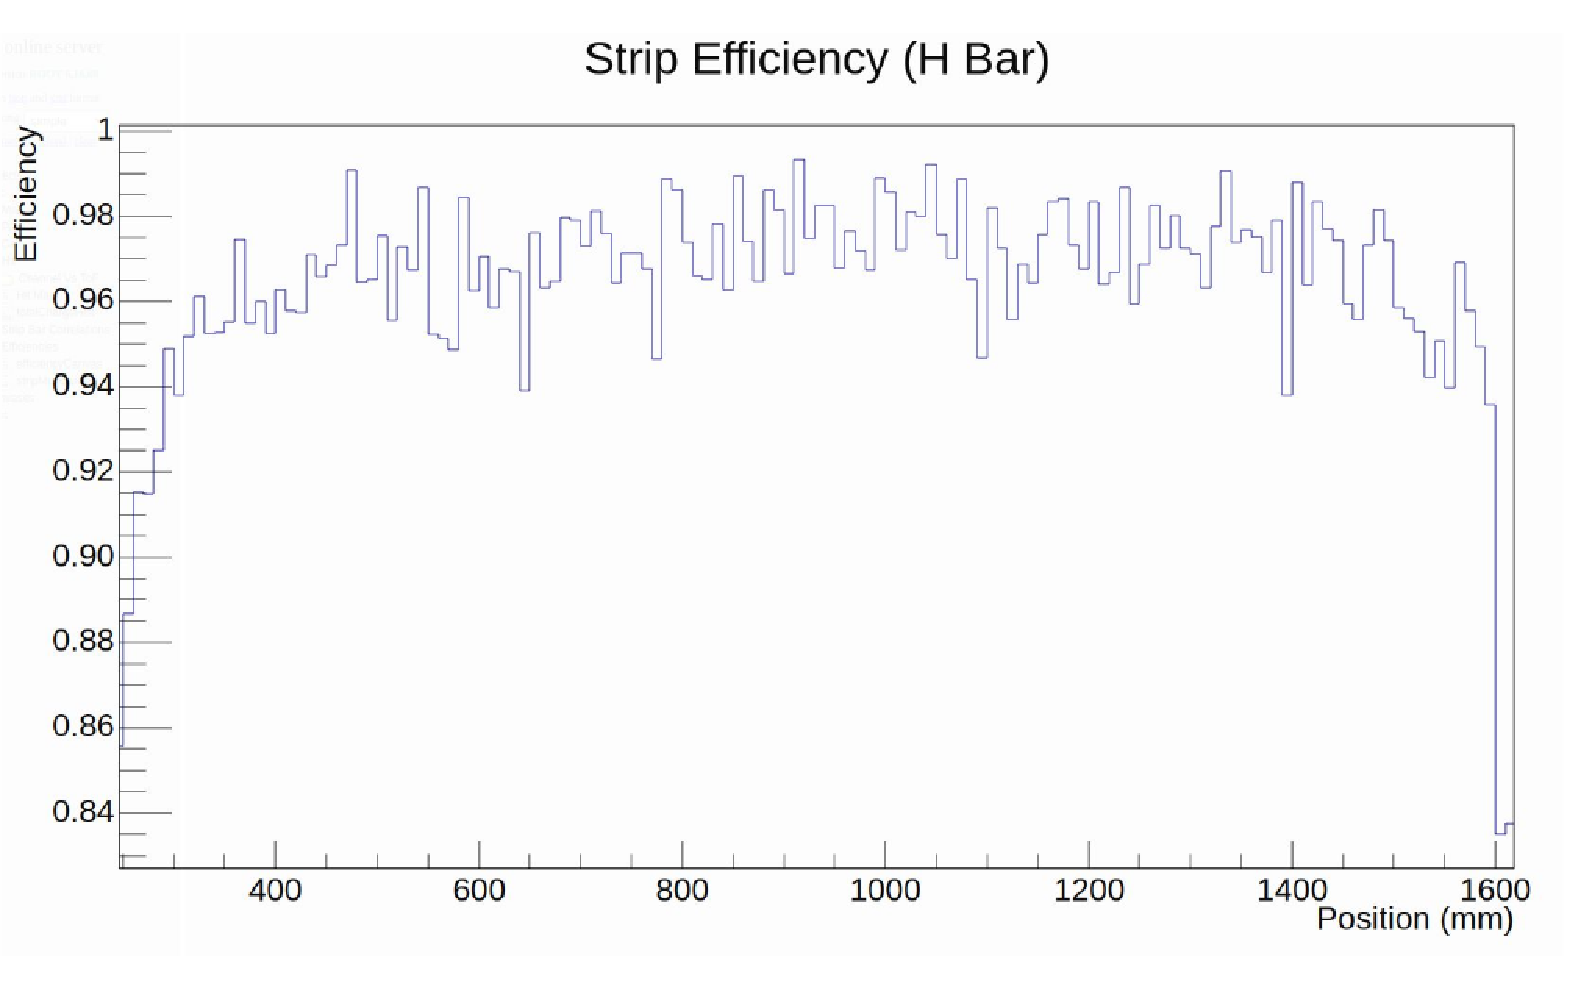
\includegraphics[width=\linewidth]{RPC Strip Efficiency}
	\caption{RPC Strip Efficiency}
	\label{fig:RPCStripEff}
\end{figure}


\section{Preparation for an Experiment}


Before each experiment
Flash the RPC with SF$_6$ to dry out the interior. An alternative (SF$_6$ is expensive) is to use Nitrogen. One has to be careful with the pressure because if it's too high it can inflate the RPC and damage it.
This process takes about a week.

When preparing to insert the gas mixture in the RPC, to check if there are no leaks, one opens the gas bottles with the mass controllers closed and then closes the bottles and checks if the pressure drops in the gas line.

Then insert the gas mixture, place one vertical NeuLAND bar on each side and calibrate in coincidence with cosmis rays. This enables us to adjust the voltage of the electrodes and find the working point of the RPC.
This process takes about a week.


\section{Calibration}